\chapter{2-nodes Algorithm}\label{chap:2-nodes}

Our model was implemented in Python 3, and is available on GitHub\footnote{\href{https://github.com/giovannt0/dpgbdt}{https://github.com/giovannt0/dpgbdt}}. Our base implementation follows \cite{dpgbdt}, with their own implementation (based on XGBoost \cite{xgboost}) available on GitHub as well\footnote{\href{https://github.com/QinbinLi/DPBoost}{https://github.com/QinbinLi/DPBoost}}. We implemented the following features:

\begin{itemize}
	\item Gradient based data filtering and geometric leaf clipping (from \cite{dpgbdt}, described in Section ~\ref{sec:query_sensitivity}). This can be enabled or disabled.
	\item Depth-first, best-leaf first and 2-nodes tree induction, outlined in Section ~\ref{sec:growth} and in this chapter.
	\item Decaying privacy budget (from \cite{wen_wang}, described in Section ~\ref{sec:budget_allocation}). This can be enabled or disabled.
\end{itemize}

\section{Design}

The 2-nodes induction method (Figure ~\ref{fig:tree_2-nodes}) is a modified version of the classical depth-first tree growth algorithm outlined in Figure ~\ref{fig:tree_dfs}. At each depth $d$ of the tree, for a given node $n_{d_i}$, $0 \leq d < d_{max}$ and $0 \leq i < 2^d$, we consider the data-points of the sibling node $n_{d_j}$ ($j$ being the index of the node that shares the same parent node as $n_{d_i}$) while computing the optimal splitting point.
The reason we opted for this design is that the exponential mechanism (used to select the splitting point) performs better the more instances there are within a node, as the gain and associated probabilities will be higher (see Equation ~\ref{eq:gbdt_gain_simplified}). By combining instances in the nodes and their siblings, we can make sure that the chosen splits will fit the data better.

\begin{figure}[h!]
	\center
	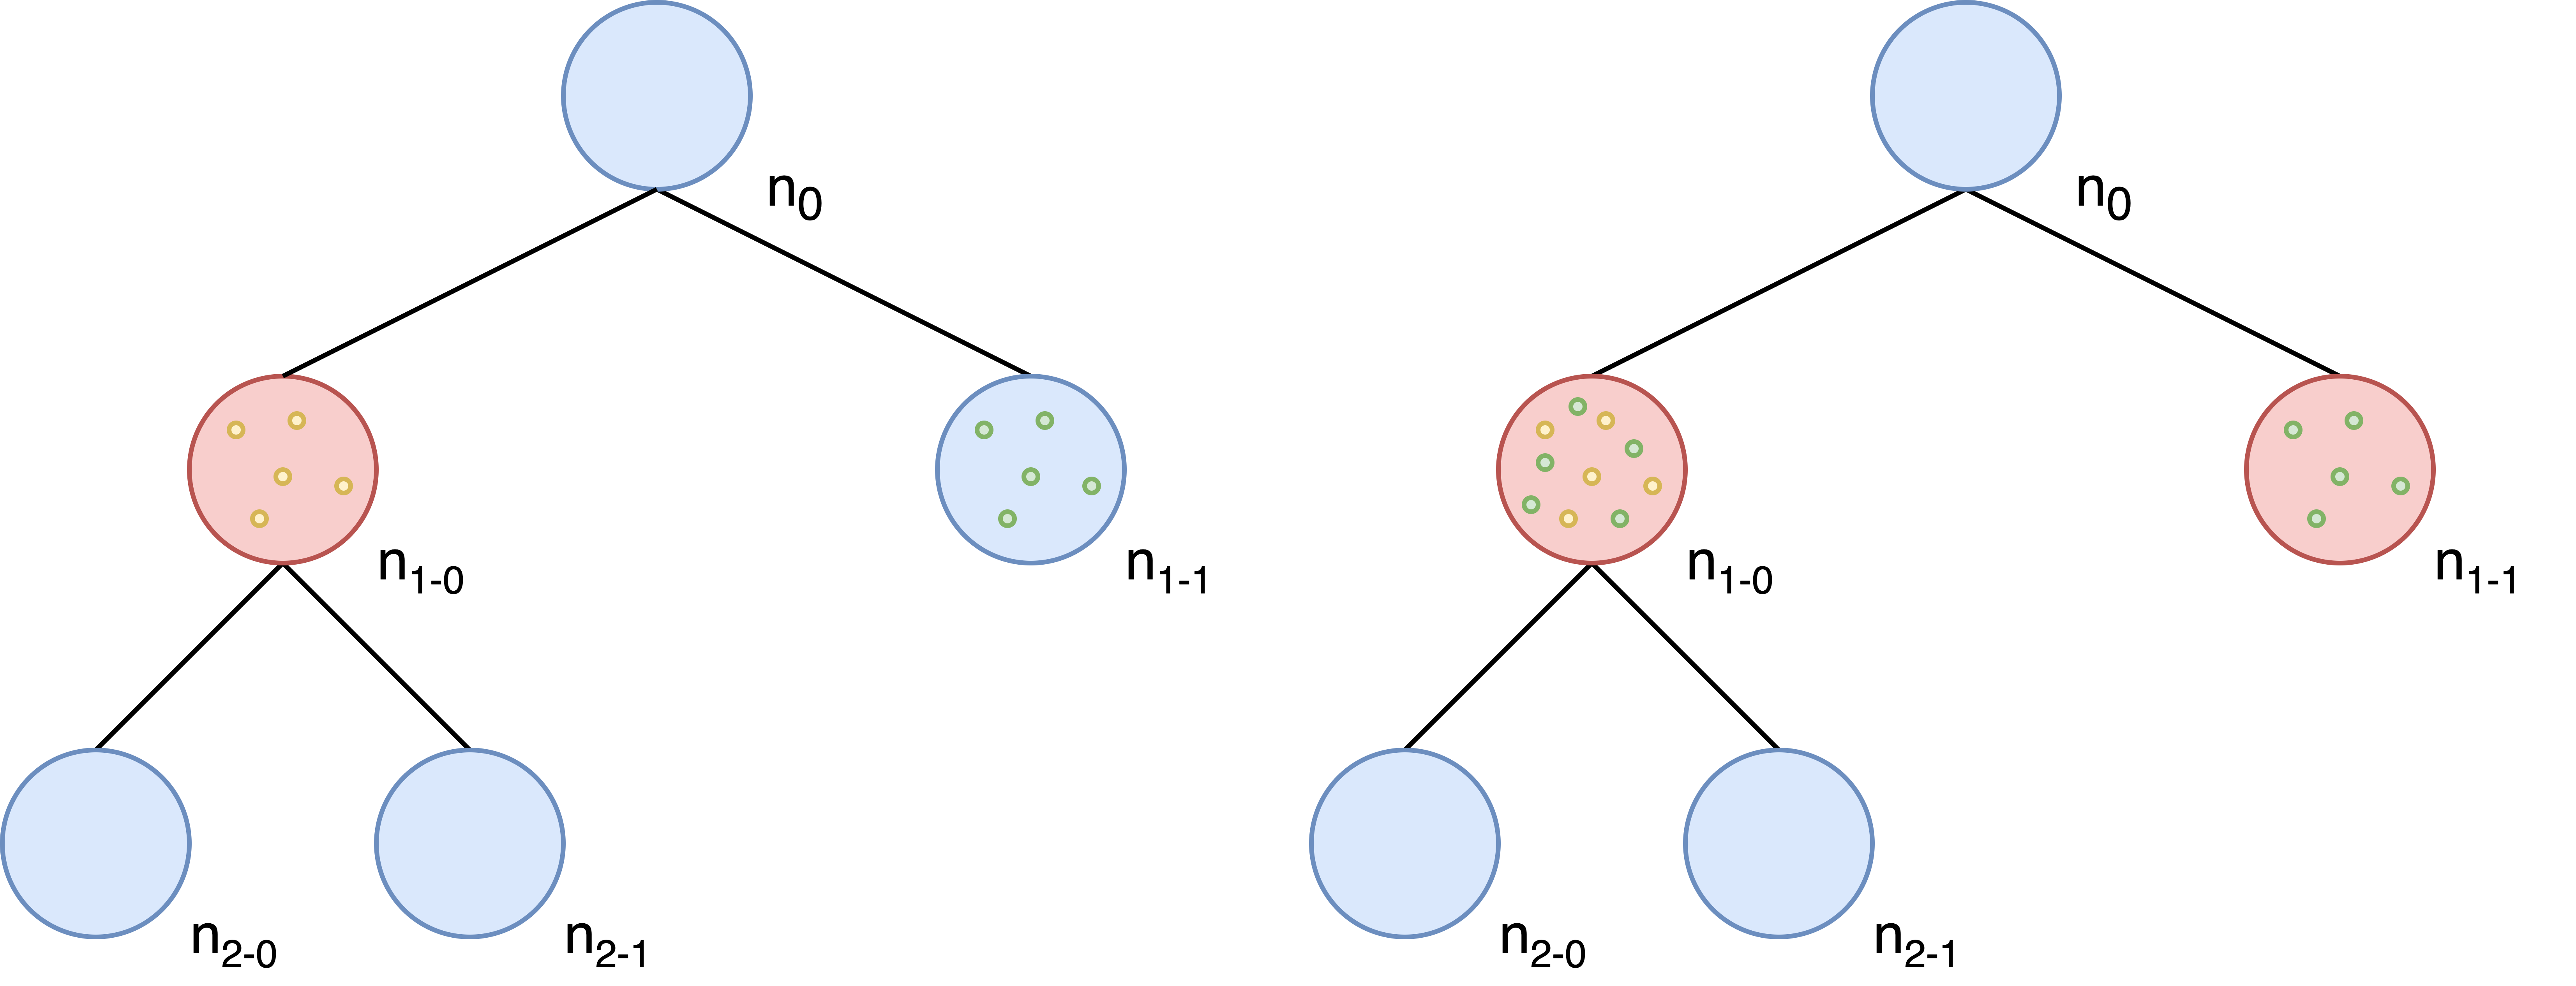
\includegraphics[scale=0.66]{images/dpgbdt/2-nodes.png}
	\caption{\label{fig:tree_2-nodes} Data-points (red nodes) being considered while splitting a node for the depth-first (left) vs. 2-nodes (right) algorithms. In the depth-first case, node $n_{1_0}$'s best split is computed over the instances of the node itself. In the 2-nodes case, node $n_{1_0}$'s best split is computed on the instances of the node itself, and the instances of its sibling node $n_{1_1}$.}
\end{figure}

\section{Properties}

In a differentially private scenario, the data-points in each node (except the root node) at every level will be queried twice (once when splitting the node, and once when splitting its sibling node). We can therefore adapt Algorithm ~\ref{algo:dp_gbdt} into Algorithm ~\ref{algo:2_nodes_dpgbdt}.

\begin{algorithm}
	\DontPrintSemicolon
	\SetKwComment{Comment}{$\triangleright$\ }{}
	\SetCommentSty{itshape}
	\caption{2-nodes DPGBDT training process}\label{algo:2_nodes_dpgbdt}
	\KwIn{$\textbf{X} = X_1,\dots,X_n$: instances, $\textbf{y} = y_1, \dots, y_n$: labels}
	\KwIn{$\lambda$: regularisation parameter, $d_{max}$: maximum depth, $\eta$: learning rate}
	\KwIn{$T$: total number of trees, $l$: loss function, $\epsilon$: privacy budget}
	\KwOut{An ensemble of trained differentially private decision trees.}
	$\epsilon_t$ = $\epsilon$ \ \Comment*[r]{\textcolor{blue}{Each tree is trained on a disjoint subset of the dataset, so we can apply Theorem ~\ref{theorem:parallel_composition}}}
	\For{$t=1$ \textbf{to} $T$}{
		Update gradients of all training instances on loss $l$ \;
		$\epsilon_{leaf} = \frac{\epsilon_t}{2}, \; \epsilon_{node} = \frac{\epsilon_t}{4d_{max}} $ \Comment*[r]{\textcolor{blue}{The budget for internal nodes is half of that in Algorithm ~\ref{algo:dp_gbdt}}}
		\For{d = 1 \textbf{to} $d_{max}$}{
			\For{\textit{each node in current depth}}{
				$g = concat(g_{node}, g_{node\_sibling})$ \Comment*[r]{\textcolor{blue}{Concat the gradients of the node and its sibling}}
				\For{\textit{each split value i}}{
					$G_i \gets \frac{(\sum_{i \in I_L}g_i)^2}{|I_L| + \lambda} + \frac{(\sum_{i \in I_R}g_i)^2}{|I_R| + \lambda}$ \Comment*[r]{\textcolor{blue}{Equation ~\ref{eq:gbdt_gain_simplified}}}
					$P_i \gets \exp(\frac{\epsilon_{node} \cdot G_i}{2 \Delta G})$ \Comment*[r]{\textcolor{blue}{Theorem ~\ref{theorem:exp}}}
				}
				Split node on split value $i$, where $i$ is chosen with probability $P_i / \sum_j P_j $
			}
		}
		\For{\textit{each leaf node i}}{
			$V_i \gets \eta \left(-\frac{\sum_{i \in I}g_i}{|I| + \lambda} + Lap(0, \Delta V/\epsilon_{leaf}) \right)$ \Comment*[r]{\textcolor{blue}{Equation ~\ref{eq:gbdt_leaf_value} and Theorem ~\ref{theorem:lap}}}
		}
	}
\end{algorithm}

\begin{theorem}
	The output of Algorithm ~\ref{algo:2_nodes_dpgbdt} satisfies \epsilon-differential privacy.
\end{theorem}
\begin{proof}
	Let $\epsilon$ be the total privacy budget for a gradient boosted decision tree model of $T$ trees. Since the trees receive a disjoint subset of the dataset, each tree receives a budget of $\epsilon_t = \epsilon$. Let $\epsilon_{leaf} = \frac{\epsilon_t}{2}$ and $\epsilon_{node} = \frac{\epsilon_t}{4d_{max}} $ be the budgets for tree $t$'s leaf nodes and its internal nodes. At each depth of the tree $t$, the inputs are disjoints and are queried exactly twice. 
	
	Per Theorem ~\ref{theorem:sequential_composition} and ~\ref{theorem:parallel_composition}, the privacy budget consumption for a single tree $t$ of depth $d_{max}$ does not exceed $\epsilon_{leaf} + 2 * d_{max} * \epsilon_{node} = \frac{\epsilon_t}{2} + 2 * d_{max} * \frac{\epsilon_t}{4*d_{max}} = \epsilon_t$. This holds for all $T$ trees, as per Theorem ~\ref{theorem:parallel_composition}. The budget consumption therefore never exceeds $\epsilon$.     
\end{proof}


Legitimately, the above algorithm raises questions regarding choosing 2 nodes to compute the gains and not a greater number. There are two main reasons for not choosing a number that is greater than 2:

\begin{enumerate}
	\item Since we query the instances $n$ times, $n$ being the number of nodes taken into account during node splitting, the privacy budget needs to be divided by $n$ as per Theorem ~\ref{theorem:sequential_composition}. For a small $\epsilon$ and a large $n$, the resulting privacy budget that is left for the nodes would be so small that there would be too much added noise in the resulting tree. This would lead to bad splits, itself leading to bad predictions.
	\item In 2-nodes, we consider the direct sibling node. The node being split and its sibling share the same parent node. This means that, up to this point in the tree, instances in both nodes are very similar, thus they can be worked on together and lead to good results. If we were to take other nodes into account, in other sub-trees that are at the same depth as the node being split, then the instances in these nodes might differ significantly. This is the case when an earlier split in the tree happens on a very distinctive attribute of the dataset. 
\end{enumerate} 

A detailed evaluation of the performances of the 2-nodes induction algorithm for both real life and synthetic datasets is given in Section ~\ref{sec:evaluation}.
